% Compile from the repository root so the screenshot paths resolve.
% Example: pdflatex -interaction=nonstopmode otp-lol-case-study.tex
\documentclass[10pt,a4paper]{article}

\usepackage[utf8]{inputenc}
\usepackage[T1]{fontenc}
\usepackage[french]{babel}
\usepackage{lmodern}
\usepackage[margin=1.55cm,headheight=14pt,footskip=20pt]{geometry}
\usepackage{graphicx}
\usepackage{xcolor}
\usepackage{tabularx}
\usepackage{array}
\usepackage{enumitem}
\usepackage{fancyhdr}
\usepackage{microtype}
\usepackage{titlesec}
\usepackage{caption}
\usepackage[hidelinks]{hyperref}

\definecolor{navy}{HTML}{101722}
\definecolor{panel}{HTML}{EEF3F8}
\definecolor{blue}{HTML}{1677D2}
\definecolor{teal}{HTML}{2BAE9B}
\definecolor{ink}{HTML}{1A2431}
\definecolor{muted}{HTML}{536273}
\definecolor{line}{HTML}{D9E2EA}

\hypersetup{
  pdftitle={OTP LOL -- étude de cas},
  pdfauthor={Quentin Chabot},
  pdfsubject={Compagnon desktop local pour League of Legends}
}
\urlstyle{same}
\renewcommand{\familydefault}{\sfdefault}
\setlength{\parindent}{0pt}
\setlength{\parskip}{5pt}
\setlist[itemize]{leftmargin=1.2em,itemsep=2pt,topsep=3pt}
\titleformat{\section}{\Large\bfseries\color{navy}}{}{0pt}{}
\titleformat{\subsection}{\normalsize\bfseries\color{blue}}{}{0pt}{}
\titlespacing*{\section}{0pt}{9pt}{4pt}
\titlespacing*{\subsection}{0pt}{6pt}{2pt}
\pagestyle{fancy}
\fancyhf{}
\fancyhead[L]{\small\textcolor{muted}{OTP LOL \textbar\ Étude de cas}}
\fancyhead[R]{\small\textcolor{muted}{Projet personnel \textbar\ octobre 2026}}
\fancyfoot[L]{\small\textcolor{muted}{Quentin Chabot}}
\fancyfoot[R]{\small\textcolor{muted}{\thepage}}

\newcommand{\tagline}[1]{{\large\color{muted}#1}}
\newcommand{\softbox}[1]{%
  \colorbox{panel}{\parbox{0.96\linewidth}{\vspace{5pt}#1\vspace{5pt}}}}
\newcommand{\smalllabel}[1]{{\small\bfseries\color{blue}\MakeUppercase{#1}}}
\newcommand{\flowstep}[2]{%
  \begin{minipage}[t]{0.225\linewidth}
    {\small\bfseries\color{blue}#1}\par\vspace{2pt}\small #2
  \end{minipage}}

\begin{document}

% 1. Couverture et écran principal.
\thispagestyle{empty}
\pagecolor{navy}
\color{white}
\vspace*{0.35cm}
{\color{teal}\rule{\textwidth}{3pt}}\par
\vspace{0.7cm}
{\small\bfseries\color{teal}COMPAGNON DES JOUEURS LEAGUE OF LEGENDS}\par
\vspace{0.28cm}
{\Huge\bfseries OTP LOL}\par
\vspace{0.16cm}
{\LARGE\bfseries Préparer ses choix. Garder le contrôle.}\par
\vspace{0.35cm}
{\large\color{white}Une application desktop Windows qui aide les joueurs à préparer leurs choix de champion et à automatiser les actions répétitives qu'ils sélectionnent dans le client League.}\par
\vspace{0.38cm}
\colorbox{white}{%
  \parbox{0.94\textwidth}{\vspace{7pt}\color{ink}
    \textbf{Pour qui ?} Pour les joueurs qui retrouvent souvent les mêmes picks, bans et équipements pendant la sélection de champion, et qui veulent préparer leurs préférences une fois puis décider eux-mêmes des automatismes à activer.
  \vspace{7pt}}}\par
\vspace{0.3cm}
\begin{center}
  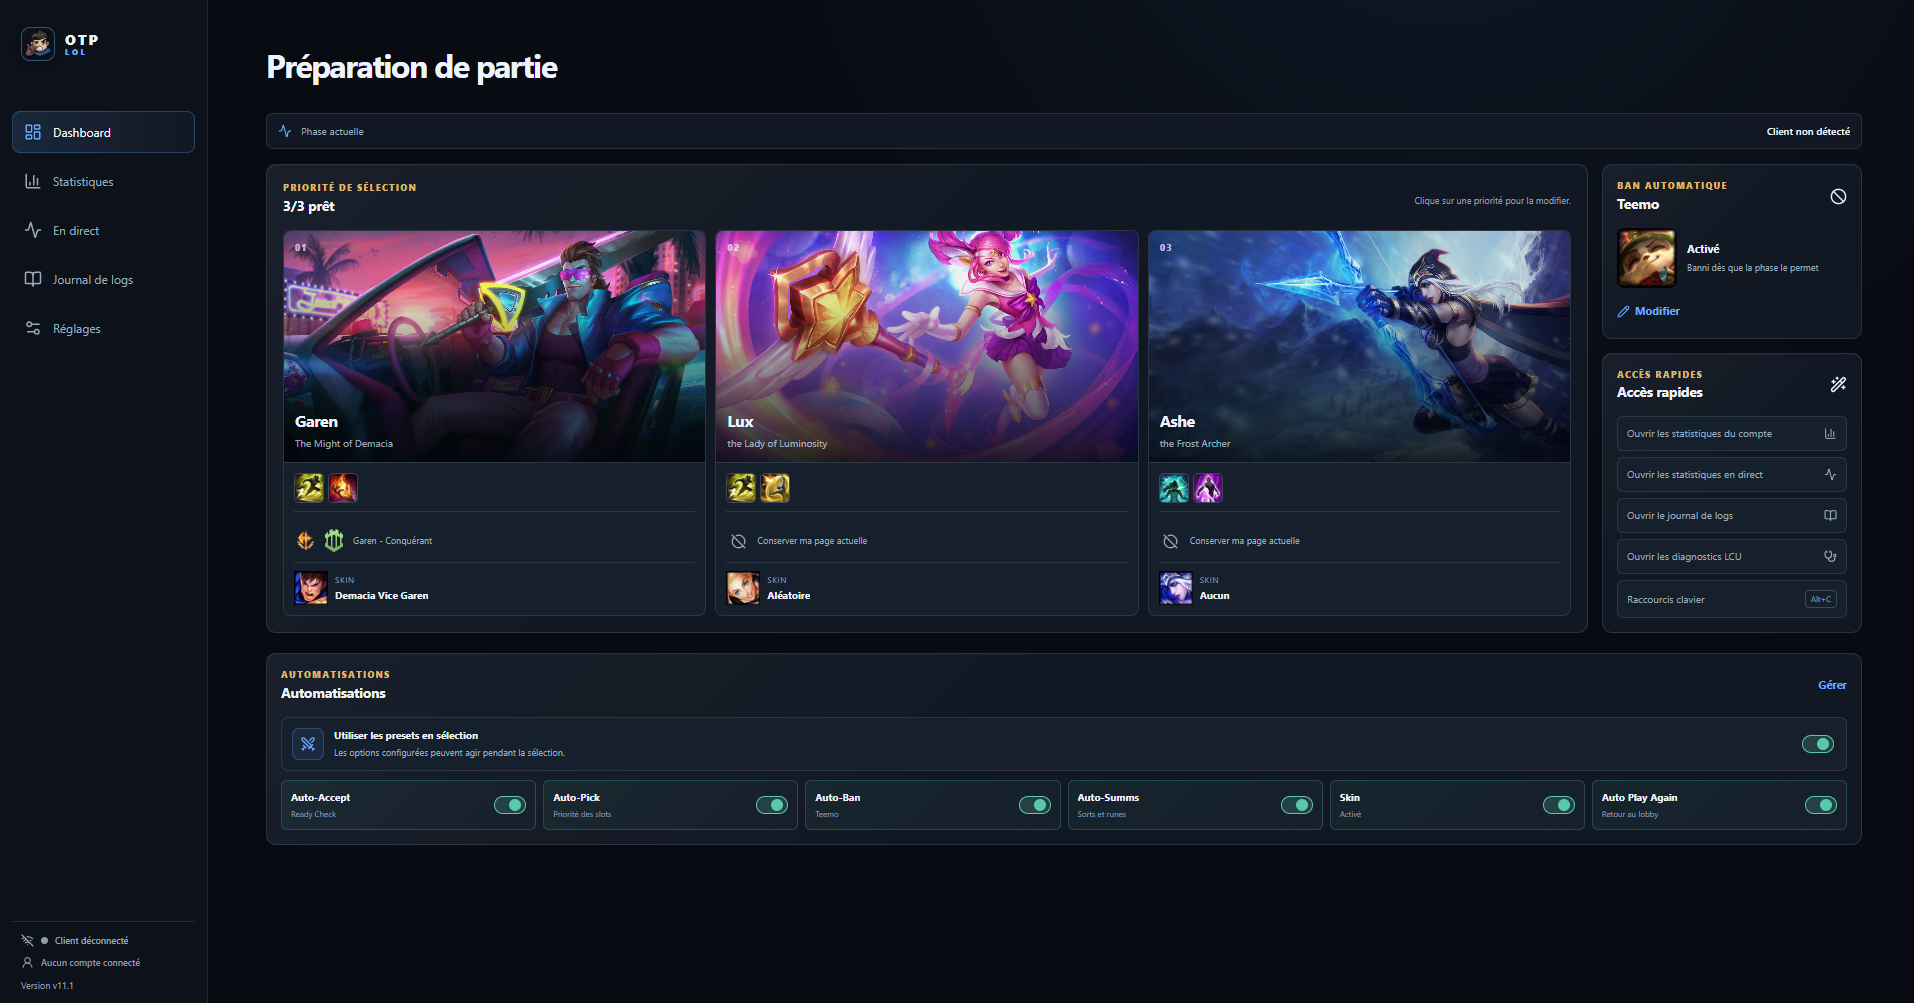
\includegraphics[width=\textwidth,height=0.47\textheight,keepaspectratio]{docs/images/portfolio-dashboard-demo.png}
\end{center}
\vspace{-2pt}
{\small\color{white}Tableau de bord de démonstration : les skins sont visibles sur les cartes. Client League déconnecté, compte absent et automatisations désactivées.}\par
\vfill
{\small\color{white}Projet personnel \textbar\ version du code 11.1 \textbar\ React + FastAPI + WebView2}\par
{\small\color{white}Capture réalisée le 14 octobre 2026 dans le parcours E2E de l'application.}\par
\newpage

% 2. Contexte, objectifs et parcours d'usage.
\pagecolor{white}
\color{ink}
\section*{Le problème et la réponse produit}
\tagline{La sélection de champion répète des choix personnels. OTP LOL les rend préparables, visibles et réutilisables.}

\subsection*{Contexte et public}
Un joueur peut retrouver les mêmes champions, sorts, runes et skins d'une partie à l'autre. Ces choix sont configurés dans le client League au fil d'une sélection courte, tandis que l'état du client change selon le lobby, la sélection, le chargement ou la fermeture du jeu. OTP LOL s'adresse aux joueurs Windows qui veulent préparer ces préférences et réduire les manipulations qu'ils répètent.

\begin{tabularx}{\textwidth}{@{}>{\bfseries}p{0.22\textwidth}X@{}}
Besoin & Retrouver rapidement un équipement associé à ses champions prioritaires.\\
Objectif & Préparer trois picks et un ban, avec sorts, runes et choix de skin configurables.\\
Principe & Chaque automatisation est contrôlable ; l'application ne joue pas la partie et ne décide pas de la stratégie du joueur.
\end{tabularx}

\subsection*{Un parcours centré sur les presets}
\begin{center}
\flowstep{01 \textbar\ Préparer}{Choisir trois priorités et un ban, même quand League est fermé.}\hfill
\flowstep{02 \textbar\ Équiper}{Associer sorts, page de runes et skin fixe ou aléatoire à chaque pick.}\hfill
\flowstep{03 \textbar\ Décider}{Activer séparément l'acceptation, le pick/ban, les sorts, les runes ou le skin.}\hfill
\flowstep{04 \textbar\ Suivre}{Voir l'état du client et les retours d'automatisation depuis le tableau de bord.}
\end{center}

\subsection*{Automatismes disponibles}
Acceptation du prêt, pick et ban prioritaires, sorts et runes, choix du skin et retour au lobby après la partie. Ces options restent désactivables dans les réglages.

\subsection*{Des écrans complémentaires, sans promesse trompeuse}
Les vues Statistiques et En direct facilitent l'ouverture d'un fournisseur tiers choisi par le joueur. Elles ne sont pas un service OTP LOL d'analyse de parties. Les réglages regroupent personnalisation, compte, raccourcis, sauvegarde de configuration et diagnostics LCU.

\vspace{3pt}
\begin{minipage}[t]{0.485\textwidth}
  \centering
  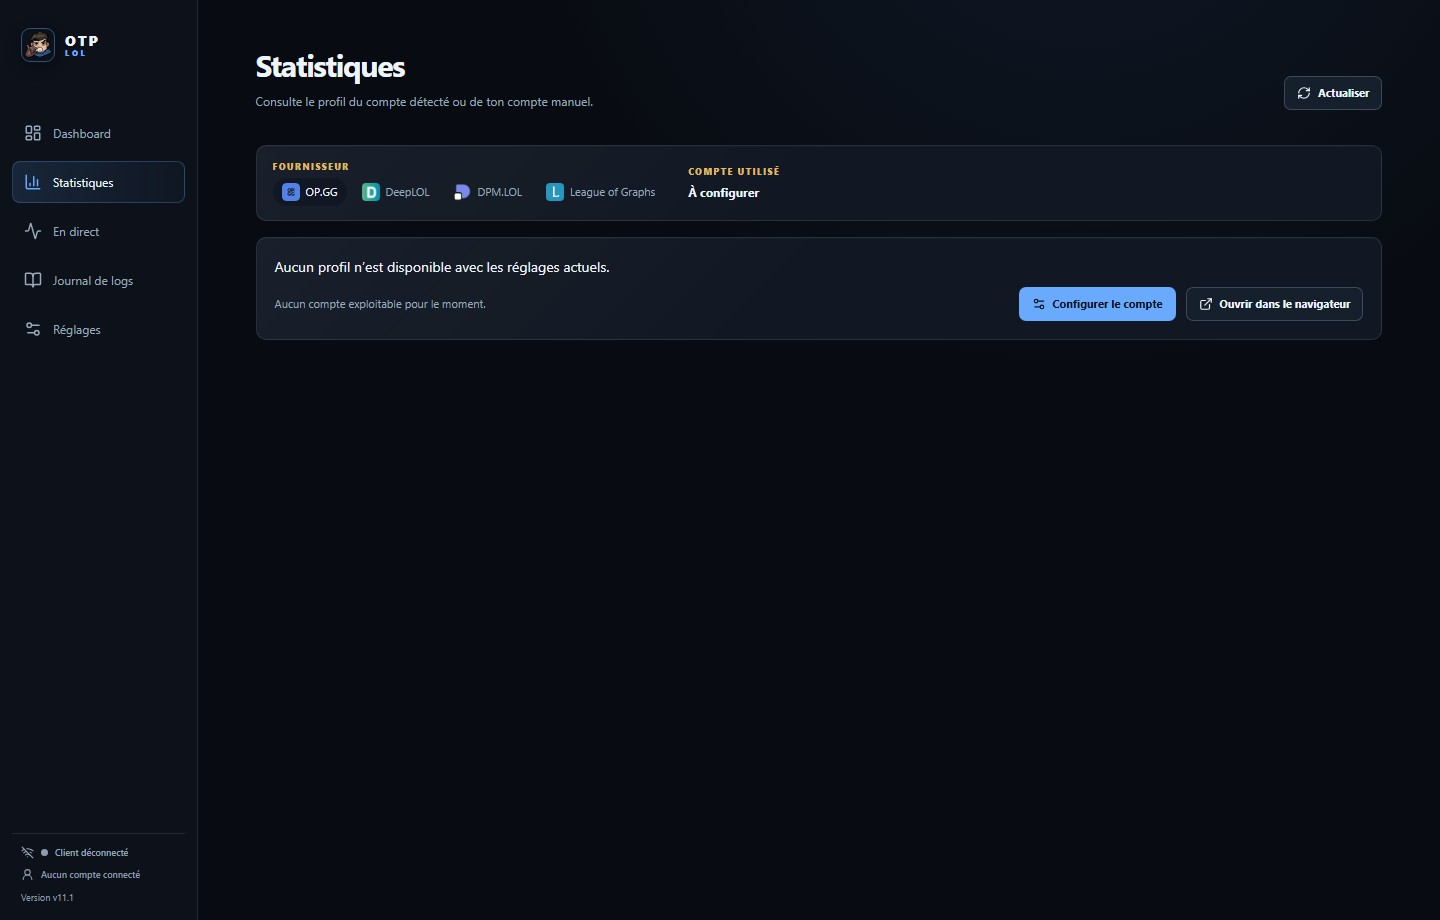
\includegraphics[width=\linewidth,height=0.23\textheight,keepaspectratio]{docs/images/portfolio-statistics-demo.jpg}
  \captionof{figure}{\small Choix du fournisseur de statistiques, sans compte connecté.}
\end{minipage}\hfill
\begin{minipage}[t]{0.485\textwidth}
  \centering
  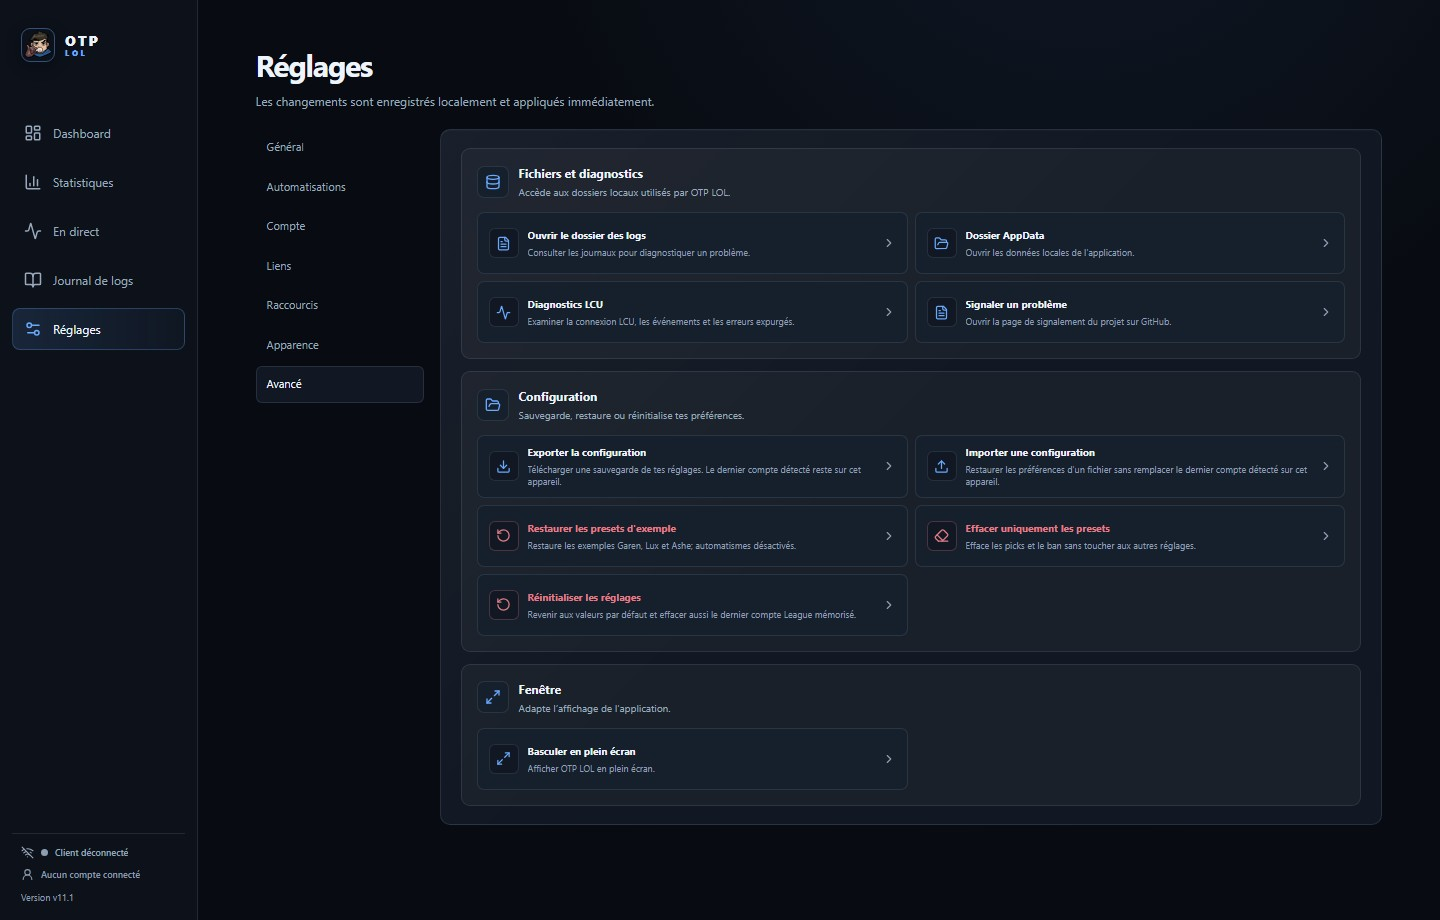
\includegraphics[width=\linewidth,height=0.23\textheight,keepaspectratio]{docs/images/portfolio-settings-demo.jpg}
  \captionof{figure}{\small Réglages avancés et diagnostics de l'application.}
\end{minipage}

{\small\color{muted}Ces captures proviennent du navigateur E2E et d'un client simulé ou déconnecté. Elles ne représentent ni une session de jeu réelle ni un compte utilisateur.}
\newpage

% 3. Architecture et technologies.
\section*{Une architecture locale, des responsabilités séparées}
\tagline{Le client League reste sur le PC. L'interface échange avec le runtime par une API locale documentée.}

\vspace{5pt}
\begin{center}
\setlength{\tabcolsep}{4pt}
\begin{tabularx}{\textwidth}{@{}>{\centering\arraybackslash}Xc>{\centering\arraybackslash}Xc>{\centering\arraybackslash}X@{}}
\softbox{\centering\textbf{React + TypeScript}\\Interface et navigation\\dans WebView2}
& $\leftrightarrow$ &
\softbox{\centering\textbf{FastAPI}\\HTTP typé + WebSocket\\sur loopback}
& $\leftrightarrow$ &
\softbox{\centering\textbf{Runtime Python}\\LCU, état de partie\\et automatismes}
\\[7pt]
& & \multicolumn{3}{c}{\softbox{\centering\textbf{Paramètres, historique et caches locaux}\quad sous \texttt{\%APPDATA\%\\OTP LOL}}} \\
\end{tabularx}
\end{center}

\begin{tabularx}{\textwidth}{@{}>{\bfseries}p{0.2\textwidth}X@{}}
Desktop & pywebview héberge le bundle React compilé dans WebView2 ; le lanceur démarre aussi l'API locale.\\
Contrat API & FastAPI et Pydantic valident les échanges ; OpenAPI alimente les types TypeScript générés.\\
État temps réel & Le backend publie les changements d'état via WebSocket ; React présente la connexion et les retours.\\
Intégration LCU & Le runtime Python gère la connexion locale, les snapshots de données de jeu et les actions autorisées.\\
Assets de jeu & Les catalogues et images utilisent les données locales du client lorsque disponibles, avec Data Dragon ou CommunityDragon comme sources de secours.
\end{tabularx}

\subsection*{Technologies et outils}
\begin{tabularx}{\textwidth}{@{}>{\bfseries}p{0.2\textwidth}X@{}}
Interface & React, TypeScript, Vite, TanStack Query et Playwright.\\
API et runtime & Python, FastAPI, Pydantic, Uvicorn, client LCU et événements WebSocket.\\
Desktop & pywebview, WebView2, intégration Windows, raccourcis et zone de notification.\\
Données & OpenAPI, fichiers de configuration locaux, historique, cache LCU et assets de jeu.\\
Livraison & GitHub Actions, build frontend et workflows de packaging Windows ; smoke desktop à valider sur Windows avec WebView2.
\end{tabularx}

\softbox{\textbf{Frontière de données.} Les réglages, l'historique et les caches restent sur le PC. OTP LOL ne requiert pas de compte applicatif ni de profil hébergé. Le jeu peut fournir des assets publics ; si le joueur ouvre un profil externe, le fournisseur choisi reçoit l'URL de ce profil.}
\newpage

% 4. Développement agentic AI-oriented et validation.
\section*{Une méthode de développement agentic AI-oriented}
\tagline{Des agents spécialisés accélèrent l'exploration et la critique ; l'intégration et les décisions restent pilotées par le développeur.}

Le projet a été développé avec une approche orientée agents IA : le travail est découpé en périmètres experts, puis leurs résultats sont confrontés avant intégration. Les agents servent à explorer le code, proposer des changements ciblés et challenger les hypothèses ; ils ne remplacent ni la revue humaine ni les preuves d'exécution.

\begin{center}
\begin{tabularx}{\textwidth}{@{}>{\centering\arraybackslash}Xc>{\centering\arraybackslash}Xc>{\centering\arraybackslash}Xc>{\centering\arraybackslash}X@{}}
\softbox{\centering\textbf{1. Cadrer}\\Entrées, contraintes et critères de réussite}
& $\rightarrow$ &
\softbox{\centering\textbf{2. Spécialiser}\\Frontend, API, LCU, desktop, sécurité, UX}
& $\rightarrow$ &
\softbox{\centering\textbf{3. Challenger}\\Revue indépendante, preuves et recherche de faux positifs}
& $\rightarrow$ &
\softbox{\centering\textbf{4. Vérifier}\\Intégration, parcours E2E et arbitrage humain}
\\
\end{tabularx}
\end{center}

\subsection*{Ce que cette approche apporte au projet}
\begin{itemize}
  \item Elle fait examiner les frontières qui concentrent le risque : React/API/OpenAPI, LCU, WebView, stockage et packaging.
  \item Des agents distincts peuvent rechercher des régressions ou contester un finding, ce qui réduit la dépendance à une seule lecture du code.
  \item Les conclusions sont ramenées à des fichiers, scénarios et validations reproductibles ; le développeur décide ce qui est exact et garde la responsabilité de l'intégration.
\end{itemize}

\subsection*{Validation technique réalisée par le projet}
Les parcours E2E lancent le frontend compilé avec un vrai processus FastAPI et WebSocket, un profil temporaire isolé et un client LCU synthétique. Ils couvrent notamment les catalogues, les presets, les événements, les transitions de connexion et des actions envoyées au faux client. Les images de la capture de couverture sont servies localement au navigateur de test ; aucun compte n'est requis.

\softbox{\textbf{Portée à ne pas surestimer.} Ces E2E ne prouvent pas le fonctionnement avec un client League réel, une fenêtre native pywebview/WebView2 installée chez l'utilisateur, le tray, les raccourcis globaux ou une release finale. Le smoke packaging Windows et le test sur un vrai client restent des validations distinctes.}
\newpage

% 5. Résultats, impact visé et suites.
\section*{Résultats, impact visé et limites}
\tagline{Une application desktop locale fonctionnelle, avec une migration vers une interface web intégrée et un contrat backend typé.}

\subsection*{Trajectoire technique}
La refonte conserve le runtime Python et l'intégration LCU tout en faisant évoluer l'interface vers React et TypeScript dans le shell desktop. FastAPI et OpenAPI rendent la frontière entre l'interface et le runtime explicite et typée.

\subsection*{Résultats livrés dans le code}
\begin{itemize}
  \item Une interface React organisée autour du dashboard, des réglages, du journal, des diagnostics et de l'accès aux fournisseurs.
  \item Un runtime Python connecté au client League local, avec des presets pour trois picks et un ban, des sorts, runes et skins.
  \item Des automatismes activables séparément, désactivés par défaut au premier lancement, avec état et retours visibles.
  \item Une frontière FastAPI/Pydantic/OpenAPI entre interface et runtime, et une persistance locale des préférences, de l'historique et des caches.
  \item Des parcours E2E full-stack qui vérifient des flux réels de l'application autour d'un client de test contrôlé.
\end{itemize}

\subsection*{Impact recherché, sans métrique inventée}
\softbox{\textbf{Pour le joueur :} réduire les manipulations répétitives autour de la sélection, retrouver ses choix plus vite et garder un contrôle explicite sur chaque automation.\\
\textbf{Pour la confidentialité :} garder les données de configuration localement et éviter d'imposer un compte OTP LOL ou un service cloud.\\
\textbf{Mesure actuelle :} le dépôt ne fournit pas de mesure d'adoption, de temps économisé, de satisfaction ou d'effet sur les résultats en jeu. Ces bénéfices sont des objectifs produit, pas des résultats quantifiés.}

\subsection*{Priorités d'une prochaine validation}
\begin{enumerate}[leftmargin=1.5em,itemsep=2pt,topsep=3pt]
  \item Exécuter le smoke du binaire final sur Windows avec WebView2 et tester le cycle natif complet : démarrage, fermeture, liens et raccourcis.
  \item Vérifier les scénarios du client League réel, notamment connexion, sélection, reconnexion et changements de version.
  \item Tester le parcours avec des joueurs, mesurer les manipulations évitées et documenter les limites des automatismes.
\end{enumerate}

\subsection*{Projet et ressources}
Code et releases : \url{https://github.com/qurnt1/otp_lol}\\
Guide de développement : \texttt{docs/development.md} \quad\textbar\quad Architecture : \texttt{docs/architecture.md}

\vfill
{\small\color{muted}OTP LOL est un projet communautaire indépendant, non affilié à Riot Games. League of Legends et les marques associées appartiennent à Riot Games.}\par
{\small\color{muted}Document préparé le 14 octobre 2026. Les interfaces sont illustrées par des données de démonstration.}

\end{document}
